\documentclass[xetex,aspectratio=169]{beamer}

\usepackage[english]{babel}
\usepackage{graphicx}
\usepackage{hyperref}
\usepackage{tikz}
%\usepackage{natbib}
\usepackage[style=authoryear, backend=bibtex]{biblatex}
\usepackage{caption}
\usepackage{subcaption}
\usepackage{multimedia}
\usepackage{amsmath}
\newcommand{\mypos}[2]{\tikz[remember picture]{\node[inner sep=0pt, anchor=base](#2){#1};}}
%\setcitestyle{authoryear,open={(},close={)}}
\DeclareMathOperator*{\argmin}{arg\,min}
\renewcommand*{\nameyeardelim}{\addcomma\space}


\usetheme{modern}

\addbibresource{biblio.bib}
\date{National Astronomy Meeting, Warwick, UK - July 15, 2022}
\title
    {High-resolution Faraday Rotation measurements}
\subtitle
    { for the MeerKAT MIGHTEE-POL Survey}
\author
    {Miguel C\'arcamo\\
    
\includegraphics[scale=0.08]{figures/logos/GitHub-Mark-120px-plus.png}\hspace{0.05cm}\href{https://www.github.com/miguelcarcamov}{\tt miguelcarcamov}\\
    
\includegraphics[scale=0.05]{figures/logos/2021 Twitter logo - blue.eps}\hspace{0.05cm}\href{https://www.twitter.com/miguel_carcamov}{\tt @miguel\_carcamov}\\
    \vspace{0.5cm}
    Anna Scaife, Russ Taylor, Matt Jarvis, Micah Bowles, Srikrishna Sekhar, Lennart Heino and Jeroen Stil\\
    }
%\logo{
\includegraphics[scale=0.5]{figures/logos/TAB_col_white_background.eps}}
\titlegraphic{\hspace{12cm}
\includegraphics[height=0.8cm, width=2cm]{figures/logos/TAB_col_white_background.eps}
}

\begin{document}

\frame[plain]{\titlepage}

%\begin{frame}{Where do cosmic magnetic fields come from?}
%\begin{columns} [onlytextwidth,t]
% Column 1
%    \begin{column}{.5\textwidth}
%       \begin{itemize}
%			\item Galaxy evolution
%			\item Star formation
%			\item Supernova remnants
%			\item Origin is \alert{\textbf{UNKNOWN}}
%		\end{itemize}
%		\begin{itemize}
%			\item Two main ways to study CMF:
%			      \begin{itemize}
%				      \item \textbf{Filaments in voids}
%				      \item Galaxy clusters
%			      \end{itemize}
%		\end{itemize}
%    \end{column}
% Column 2
%\begin{column}{.5\textwidth}
%    \begin{figure}
%        \centering
%         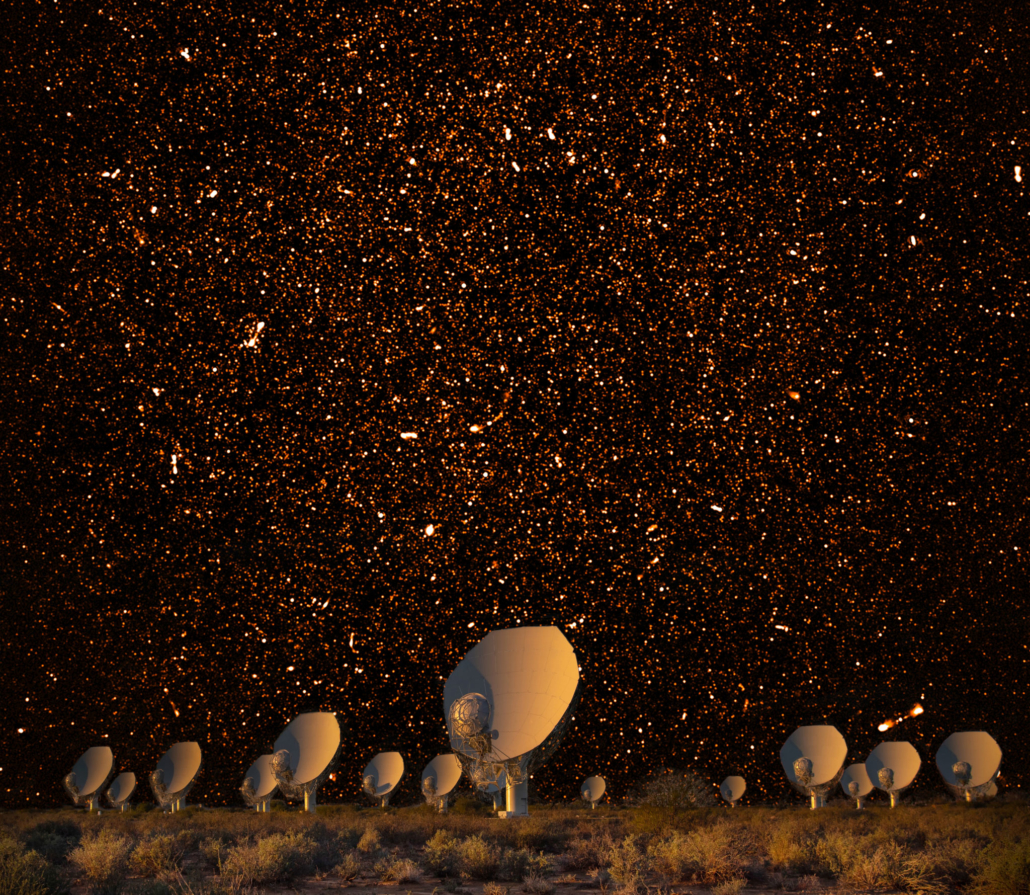
\includegraphics[width=\textwidth]{figures/MeerKATDeep2_compositeV6.jpg}
%        \caption*{Credit: SARAO}
%     \end{figure}
%\end{column}%

%\end{columns}

% \end{frame}
\begin{frame}<0>{Studying magnetic fields using Faraday Rotation}
	\begin{figure}
		\centering
		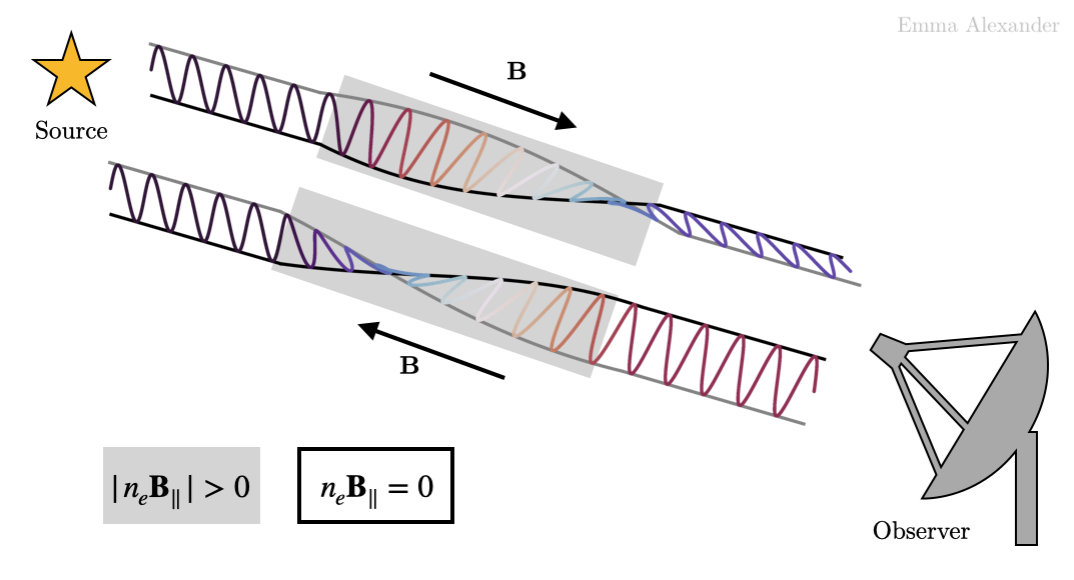
\includegraphics[width=.8\textwidth]{figures/faraday_rot.png}
		\caption*{Faraday rotation illustration. Credit: \href{https://emmaalexander.github.io/resources.html}{Emma Alexander}.}
	\end{figure}
\end{frame}

\begin{frame}{Studying magnetic fields using Faraday Rotation}
	\footnotesize
	\begin{columns}

		\begin{column}{0.55\textwidth}
			%The RM Synthesis method exploits a Fourier relationship between polarisation intensity ($P$) as a function of wavelength squared and the Faraday dispersion function to recover polarised intensity as a function of Faraday depth $\phi$ along a line of sight (LOS)

			%\begin{equation}
			%	\label{eq:fourier}
			%	F(\phi) = \int_{-\infty}^{\infty}{ P(\lambda^2){\rm e}^{-2i\phi \lambda^2}~{\rm d}\lambda^2 },
			%\end{equation}

			%where
			%
			%\begin{equation}
			%	\label{eq:pol}
			%	P(\lambda^2) = |P(\lambda^2)|{\rm e}^{2i\chi(\lambda^2)} = Q(\lambda^2) + iU(\lambda^2).
			%\end{equation}

			\begin{block}{Rotation Measure}
				\begin{equation*}
					\text{RM} = 0.81 \int_{\text{source}}^{\text{observer}} n_e(r) B_{||}(r) \cdot dr\; \text{rad}\;\text{m}^{-2}
				\end{equation*}
			\end{block}

		\end{column}

		\begin{column}{0.45\textwidth}
			\begin{figure}
				\centering
				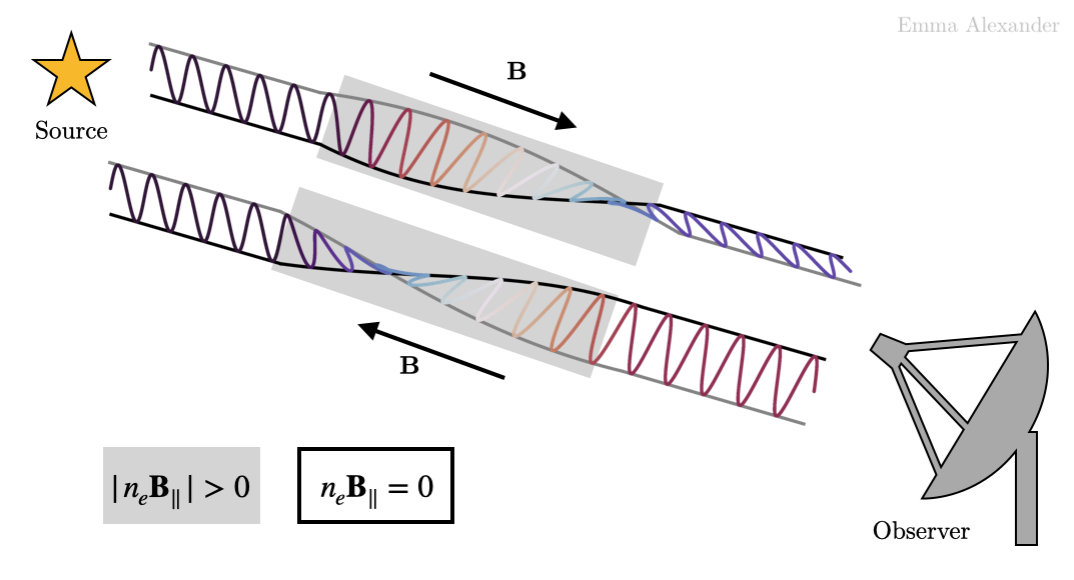
\includegraphics[width=\textwidth]{figures/faraday_rot.png}
				\caption*{Faraday rotation illustration. Credit: \href{https://emmaalexander.github.io/resources.html}{Emma Alexander}.}
			\end{figure}
		\end{column}
	\end{columns}

\end{frame}

\begin{frame}{Studying magnetic fields using Faraday Rotation}
	\footnotesize
	\begin{columns}

		\begin{column}{0.55\textwidth}
			%The RM Synthesis method exploits a Fourier relationship between polarisation intensity ($P$) as a function of wavelength squared and the Faraday dispersion function to recover polarised intensity as a function of Faraday depth $\phi$ along a line of sight (LOS)

			%\begin{equation}
			%	\label{eq:fourier}
			%	F(\phi) = \int_{-\infty}^{\infty}{ P(\lambda^2){\rm e}^{-2i\phi \lambda^2}~{\rm d}\lambda^2 },
			%\end{equation}

			%where
			%
			%\begin{equation}
			%	\label{eq:pol}
			%	P(\lambda^2) = |P(\lambda^2)|{\rm e}^{2i\chi(\lambda^2)} = Q(\lambda^2) + iU(\lambda^2).
			%\end{equation}

			\begin{block}{Rotation Measure}
				\begin{equation*}
					\mypos{\text{RM}}{rm} = 0.81 \int_{\text{source}}^{\text{observer}} \mypos{$n_e$}{ne}(r) \mypos{$B_{||}$}{be}(r) \cdot dr\; \text{rad}\;\text{m}^{-2}
				\end{equation*}
			\end{block}

			\begin{equation*}
				\label{eq:fourier}
				F(\phi) = \frac{1}{K} \int_{-\infty}^{\infty}{ W(\lambda^2)P(\lambda^2){\rm e}^{-2i\phi \lambda^2}~{\rm d}\lambda^2 },
			\end{equation*}
			\begin{equation*}
				\label{eq:pol}
				\mypos{$P(\lambda^2)$}{ppos} = |P(\lambda^2)|{\rm e}^{2i\chi(\lambda^2)} = Q(\lambda^2) + iU(\lambda^2).
			\end{equation*}
		\end{column}

		\begin{column}{0.45\textwidth}
			\begin{figure}
				\centering
				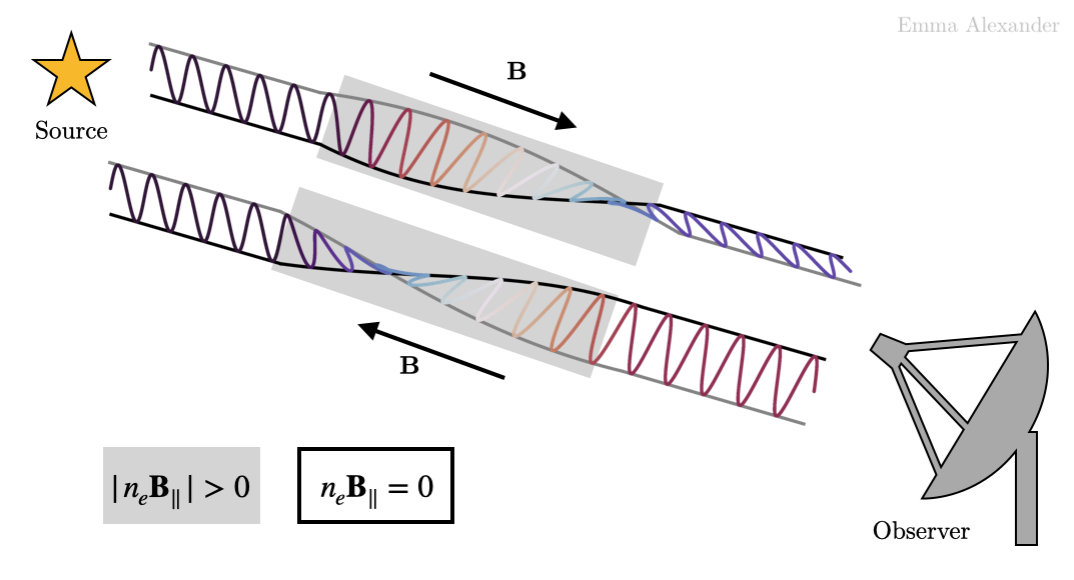
\includegraphics[width=\textwidth]{figures/faraday_rot.png}
				\caption*{Faraday rotation illustration. Credit: \href{https://emmaalexander.github.io/resources.html}{Emma Alexander}.}
			\end{figure}
		\end{column}
	\end{columns}
	\begin{tikzpicture}[overlay, remember picture, scale=0.7]
		\node[draw, modernRed, circle, very thick, minimum size=20pt, opacity=0.3] (A) at (rm){};
		\node[draw, modernRed, circle, very thick, minimum size=20pt, opacity=0.3] (B) at (ne){};
		\node[draw, modernRed, circle, very thick, minimum size=20pt, opacity=0.3] (C) at (be){};
		\draw[->, modernRed, very thick, opacity=0.3] (A.south west) to[bend right] ++(1,-1) node[modernRed, anchor=west] (Atext) {Radio};
		\draw[->, modernRed, very thick, opacity=0.3] (B.south) to[bend right] ++(1,-1) node[modernRed, anchor=west] (Btext) {X-Ray};
		\draw[->, modernRed, very thick, opacity=0.3] (C.north west) to[bend left] ++(1,0.5) node[modernRed, anchor=west] (Ctext) {\textbf{What we want}};
		\draw[->, modernRed, very thick, opacity=0.3] (Atext.south west) to [bend right] ++(-1.,-1.5) node[modernRed!80, anchor=west] (ppos) {};
	\end{tikzpicture}
\end{frame}

\begin{frame}<0>{MeerKAT}
	\begin{columns}[onlytextwidth,t]
		% Column 1
		\begin{column}{.5\textwidth}
			\begin{itemize}
				\item Square Kilometre Array (SKA) precursor
				\item 64 antennas
				\item Dish diameter: 13.5 m
				\item Baselines from 29 m to 7700 m
				\item Frequency range [L-band]: 900 - 1670 MHz
				\item Resolution $\sim$ 9''
			\end{itemize}
		\end{column}
		% Column 2
		\begin{column}{.5\textwidth}
			\begin{figure}
				\centering
				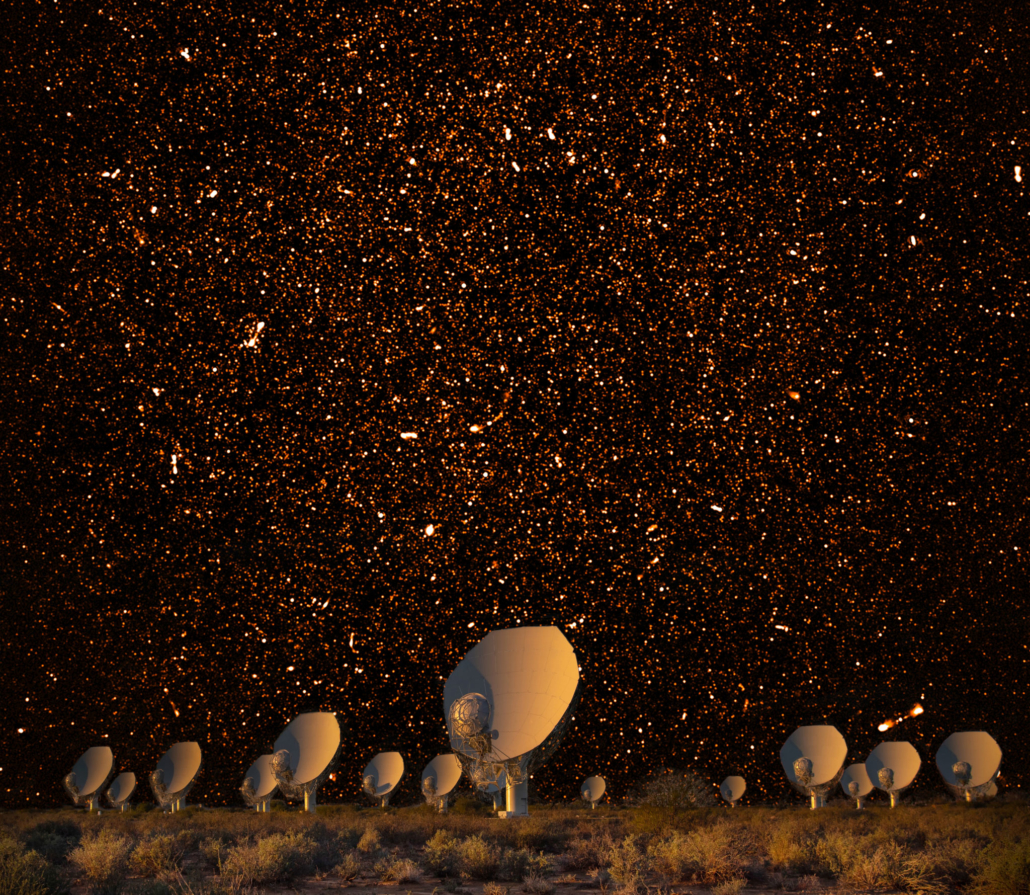
\includegraphics[width=\textwidth]{figures/MeerKATDeep2_compositeV6.jpg}
				\caption*{Credit: SARAO}
			\end{figure}
		\end{column}%

	\end{columns}
\end{frame}

\begin{frame}{THE MIGHTEE-POL survey [Early science]}
	\begin{columns}[onlytextwidth,t]
		% Column 1
		\begin{column}{.5\textwidth}
			\textbf{COSMOS}
			\begin{itemize}
				\item 17.45\;hrs observation
				\item 1.6\;deg$^{2}$
				\item Noise: 1.7\;$\mu$Jy/beam
				\item  Resolution: 8.6''
				\item 9,896 sources
			\end{itemize}
		\end{column}
		% Column 2
		\begin{column}{.5\textwidth}
			\begin{figure}
				\centering
				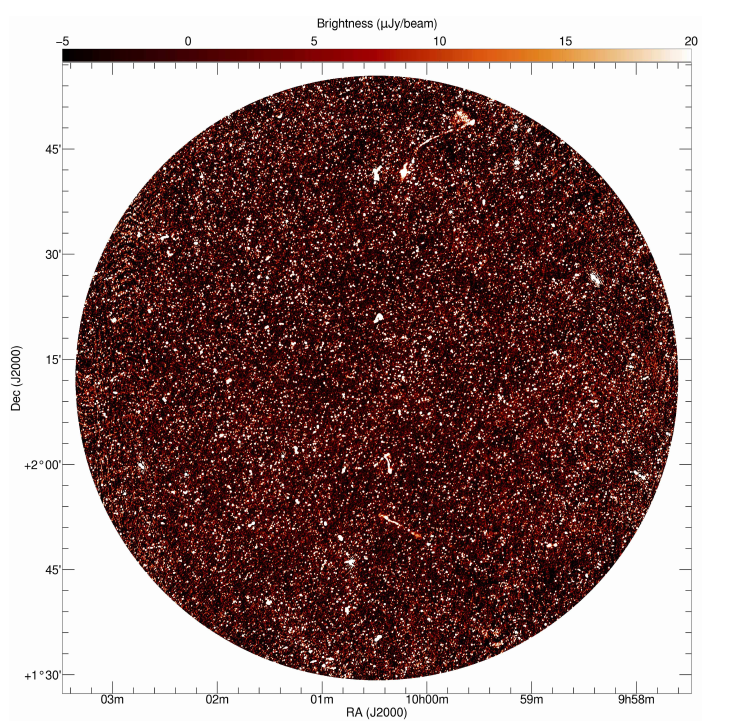
\includegraphics[scale=0.2]{figures/mightee_survey/cosmos.png}
				\caption*{COSMOS Stokes I Continuum map ~\parencite{mightee-pol}}
				\label{fig:cosmos}
			\end{figure}
		\end{column}%

	\end{columns}

\end{frame}

\begin{frame}{THE MIGHTEE-POL survey [Early science]}
	\begin{columns}[onlytextwidth,t]
		% Column 1
		% Column 2
		\begin{column}{.5\textwidth}
			\textbf{XMMLSS}
			\begin{itemize}
				\item 16.05, 16.12, 16.03 hrs observation
				\item Three fields that cover 3.5\;deg$^{2}$
				\item Resolution: 8.2''
				\item 20,274 sources
			\end{itemize}

		\end{column}

		\begin{column}{.5\textwidth}
			\begin{figure}
				\centering
				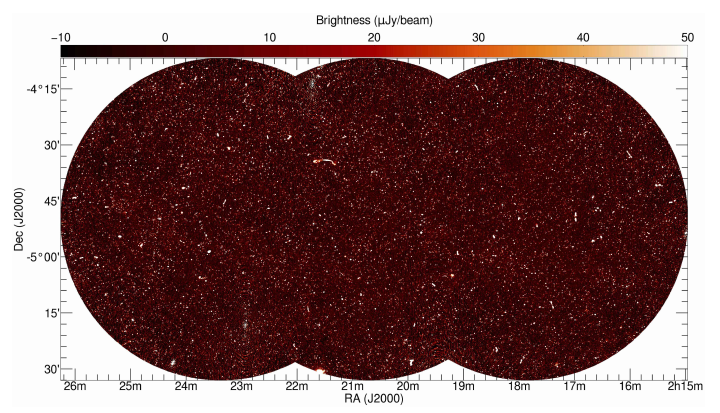
\includegraphics[scale=0.3]{figures/mightee_survey/xmmlss.png}
				\caption*{XMMLSS Stokes I Continuum mosaic map ~\parencite{mightee-pol}}
				\label{fig:xmmlss}
			\end{figure}
		\end{column}

	\end{columns}
\end{frame}


\begin{frame}<0>{CS-ROMER: Compressed Sensing ROtation MEasure Reconstruction}
	\begin{figure}
		\centering
		
\includegraphics[width=0.2\textwidth]{figures/logos/GitHub-Mark-120px-plus.png}
		%\caption{Caption}
		%\label{fig:my_label}
	\end{figure}

	\begin{center}
		\url{http://github.com/miguelcarcamov/csromer}
	\end{center}


\end{frame}


\begin{frame}{CS-ROMER: Compressed Sensing ROtation MEasure Reconstruction}
	\begin{columns}[onlytextwidth,t]
		% Column 1
		\begin{column}{.5\textwidth}
			\begin{figure}
				\centering
				
\includegraphics[scale=0.5]{figures/logos/GitHub-Mark-120px-plus.png}
				%\caption{Caption}
				%\label{fig:my_label}
			\end{figure}

			\url{http://github.com/miguelcarcamov/csromer}
		\end{column}
		% Column 2
		\begin{column}{.5\textwidth}
			\begin{itemize}
				\item Reconstruction of Faraday depth sources from linearly polarized data with CS

			\end{itemize}
		\end{column}%

	\end{columns}
\end{frame}

\begin{frame}{CS-ROMER: Compressed Sensing ROtation MEasure Reconstruction}
	\begin{columns}[onlytextwidth,t]
		% Column 1
		\begin{column}{.5\textwidth}
			\begin{figure}
				\centering
				
\includegraphics[scale=0.5]{figures/logos/GitHub-Mark-120px-plus.png}
				%\caption{Caption}
				%\label{fig:my_label}
			\end{figure}

			\url{http://github.com/miguelcarcamov/csromer}
		\end{column}
		% Column 2
		\begin{column}{.5\textwidth}
			\begin{itemize}
				\item Reconstruction of Faraday depth sources from linearly polarized data with CS
				\item More than 100 wavelet filters provided by {\tt Pywavelets}

			\end{itemize}
		\end{column}%

	\end{columns}
\end{frame}

\begin{frame}{CS-ROMER: Compressed Sensing ROtation MEasure Reconstruction}
	\begin{columns}[onlytextwidth,t]
		% Column 1
		\begin{column}{.5\textwidth}
			\begin{figure}
				\centering
				
\includegraphics[scale=0.5]{figures/logos/GitHub-Mark-120px-plus.png}
				%\caption{Caption}
				%\label{fig:my_label}
			\end{figure}

			\url{http://github.com/miguelcarcamov/csromer}
		\end{column}
		% Column 2
		\begin{column}{.5\textwidth}
			\begin{itemize}
				\item Reconstruction of Faraday depth sources from linearly polarized data with CS
				\item More than 100 wavelet filters provided by {\tt Pywavelets}
				\item Simulation of Faraday depth sources directly in $\lambda^2$-space

			\end{itemize}
		\end{column}%

	\end{columns}
\end{frame}

\begin{frame}{CS-ROMER: Compressed Sensing ROtation MEasure Reconstruction}
	\begin{columns}[onlytextwidth,t]
		% Column 1
		\begin{column}{.5\textwidth}
			\begin{figure}
				\centering
				
\includegraphics[scale=0.5]{figures/logos/GitHub-Mark-120px-plus.png}
				%\caption{Caption}
				%\label{fig:my_label}
			\end{figure}

			\url{http://github.com/miguelcarcamov/csromer}
		\end{column}
		% Column 2
		\begin{column}{.5\textwidth}
			\begin{itemize}
				\item Reconstruction of Faraday depth sources from linearly polarized data with CS
				\item More than 100 wavelet filters provided by {\tt Pywavelets}
				\item Simulation of Faraday depth sources directly in $\lambda^2$-space
				\item Subtraction of Galactic RM

			\end{itemize}
		\end{column}%

	\end{columns}
\end{frame}

\begin{frame}{CS-ROMER: Compressed Sensing ROtation MEasure Reconstruction}
	\begin{columns}[onlytextwidth,t]
		% Column 1
		\begin{column}{.5\textwidth}
			\begin{figure}
				\centering
				
\includegraphics[scale=0.5]{figures/logos/GitHub-Mark-120px-plus.png}
				%\caption{Caption}
				%\label{fig:my_label}
			\end{figure}

			\url{http://github.com/miguelcarcamov/csromer}
		\end{column}
		% Column 2
		\begin{column}{.5\textwidth}
			\begin{itemize}
				\item Reconstruction of Faraday depth sources from linearly polarized data with CS
				\item More than 100 wavelet filters provided by {\tt Pywavelets}
				\item Simulation of Faraday depth sources directly in $\lambda^2$-space
				\item Subtraction of Galactic RM
				\item Spectral index correction
			\end{itemize}
		\end{column}%

	\end{columns}
\end{frame}

\begin{frame}{Simulation of Faraday sources}
	\begin{itemize}
		\item Simulation of thin, thick or mixed/complex sources
		\item Simulation of RFI flagging
		\item Noise application to simulated data
	\end{itemize}

\end{frame}



\begin{frame}<0>{Thin, thick, mixed/complex sources}

	\begin{figure}
		\centering

		\begin{subfigure}{0.2\textwidth}
			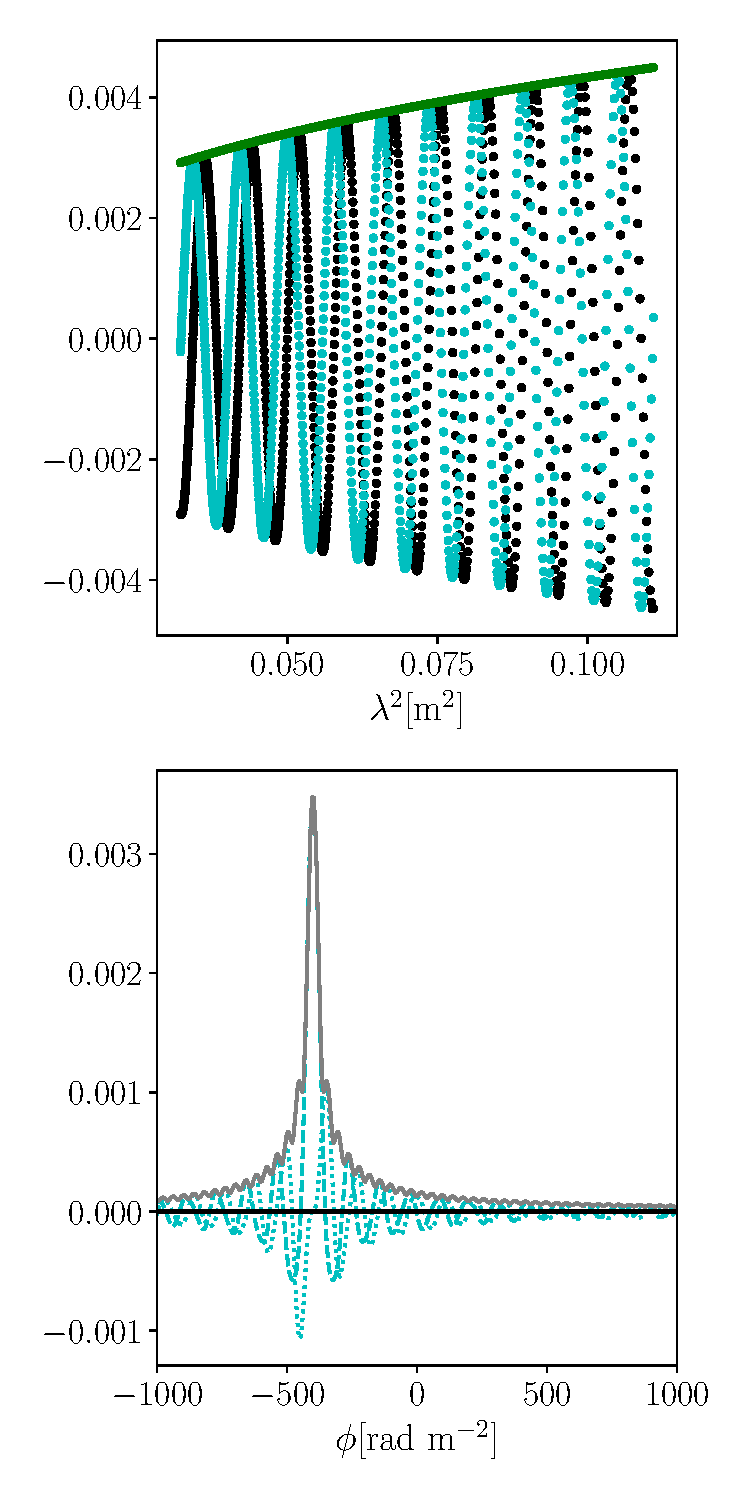
\includegraphics[width=\textwidth]{figures/sources/thin_source.pdf}
			\caption{Thin source}
		\end{subfigure}
		\begin{subfigure}{0.2\textwidth}
			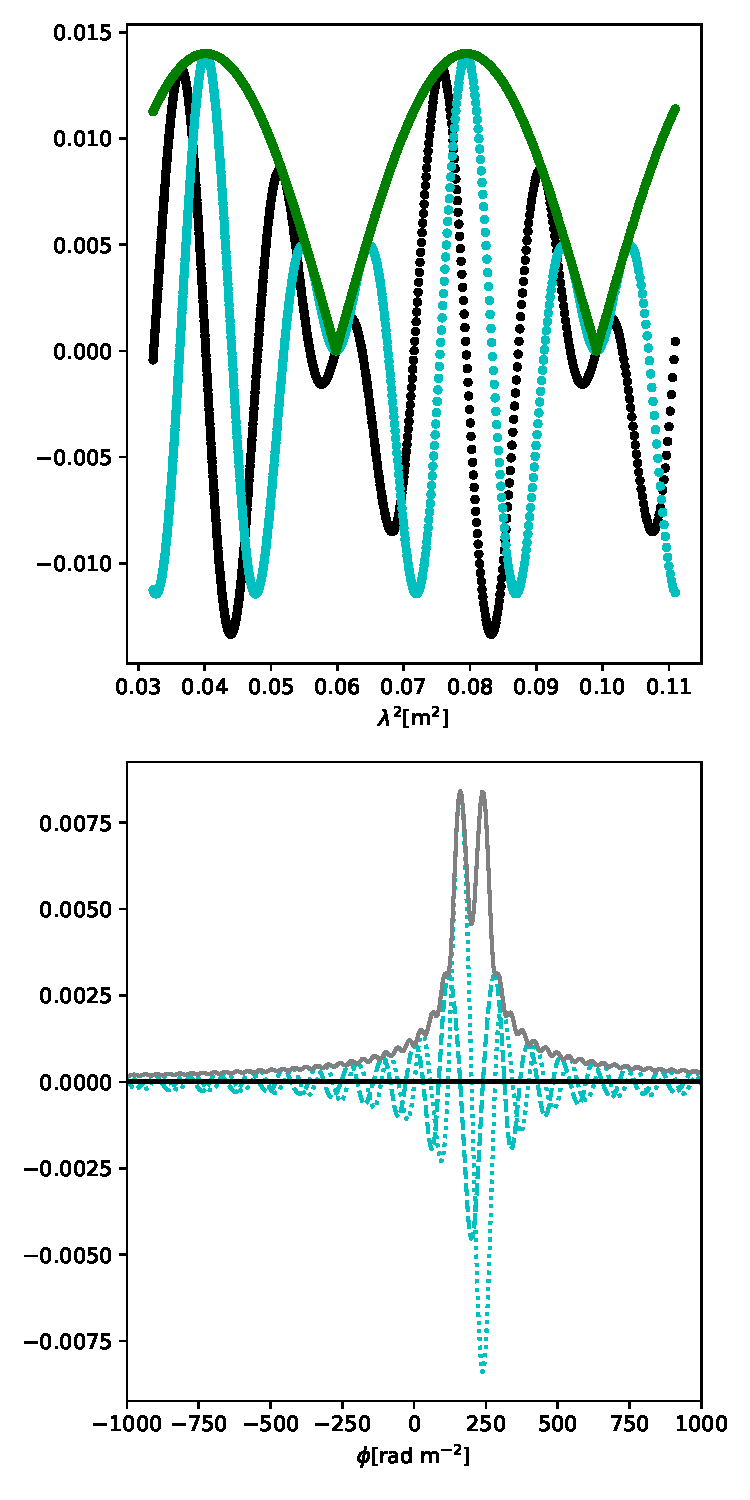
\includegraphics[width=\textwidth]{figures/sources/thick_source.pdf}
			\caption{Thick source}
		\end{subfigure}
		\begin{subfigure}{0.2\textwidth}
			%\vspace{0.4cm}
			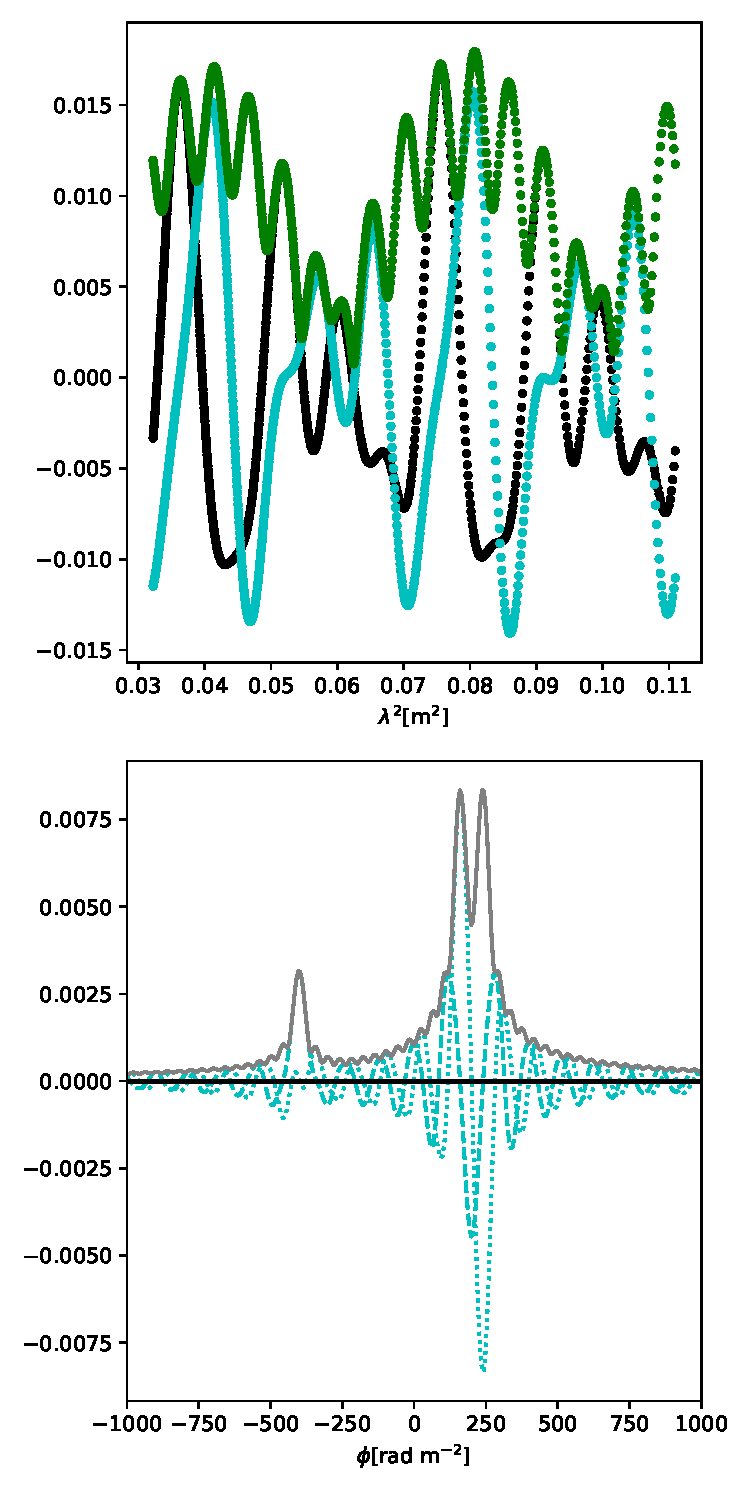
\includegraphics[width=\textwidth]{figures/sources/mixed_source.pdf}
			\caption{Complex source}
		\end{subfigure}
	\end{figure}

\end{frame}

\begin{frame}<0>{RFI \& noise example}

	\begin{figure}
		\centering

		\begin{subfigure}{0.2\textwidth}
			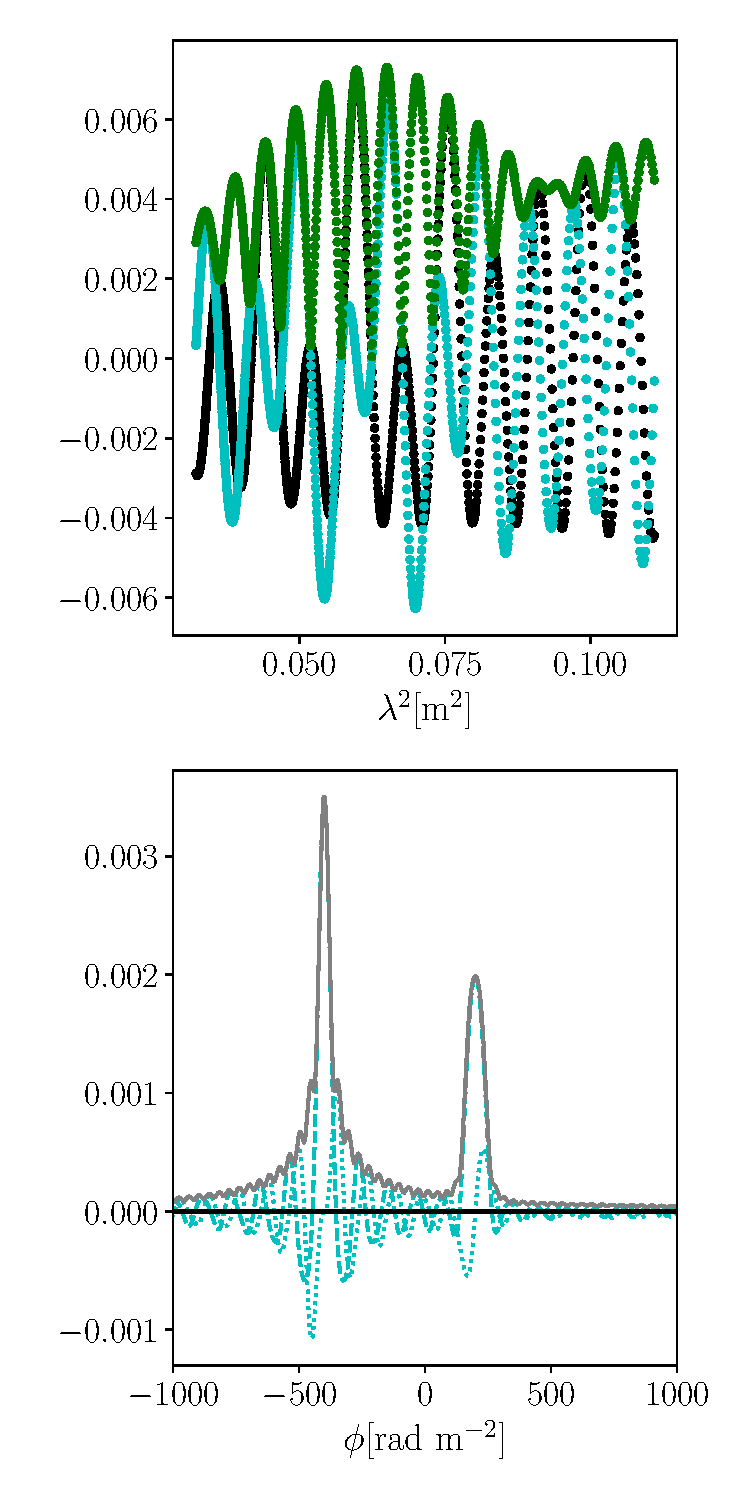
\includegraphics[width=\textwidth]{figures/dataset_features/data_normal.pdf}
			\caption{Complete dataset}
		\end{subfigure}
		\begin{subfigure}{0.2\textwidth}
			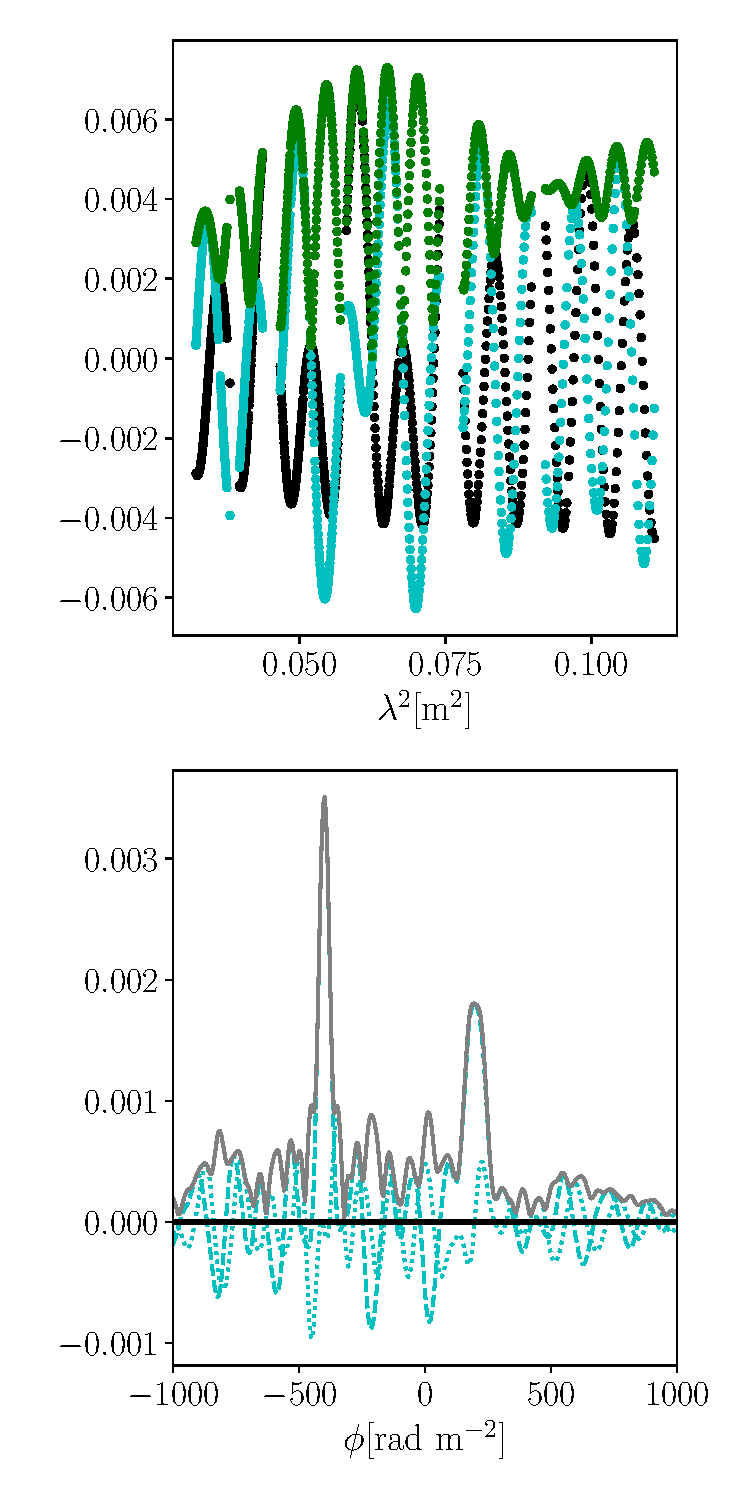
\includegraphics[width=\textwidth]{figures/dataset_features/data_removed.pdf}
			\caption{20\% data removed}
		\end{subfigure}
		\begin{subfigure}{0.2\textwidth}
			%\vspace{0.1cm}
			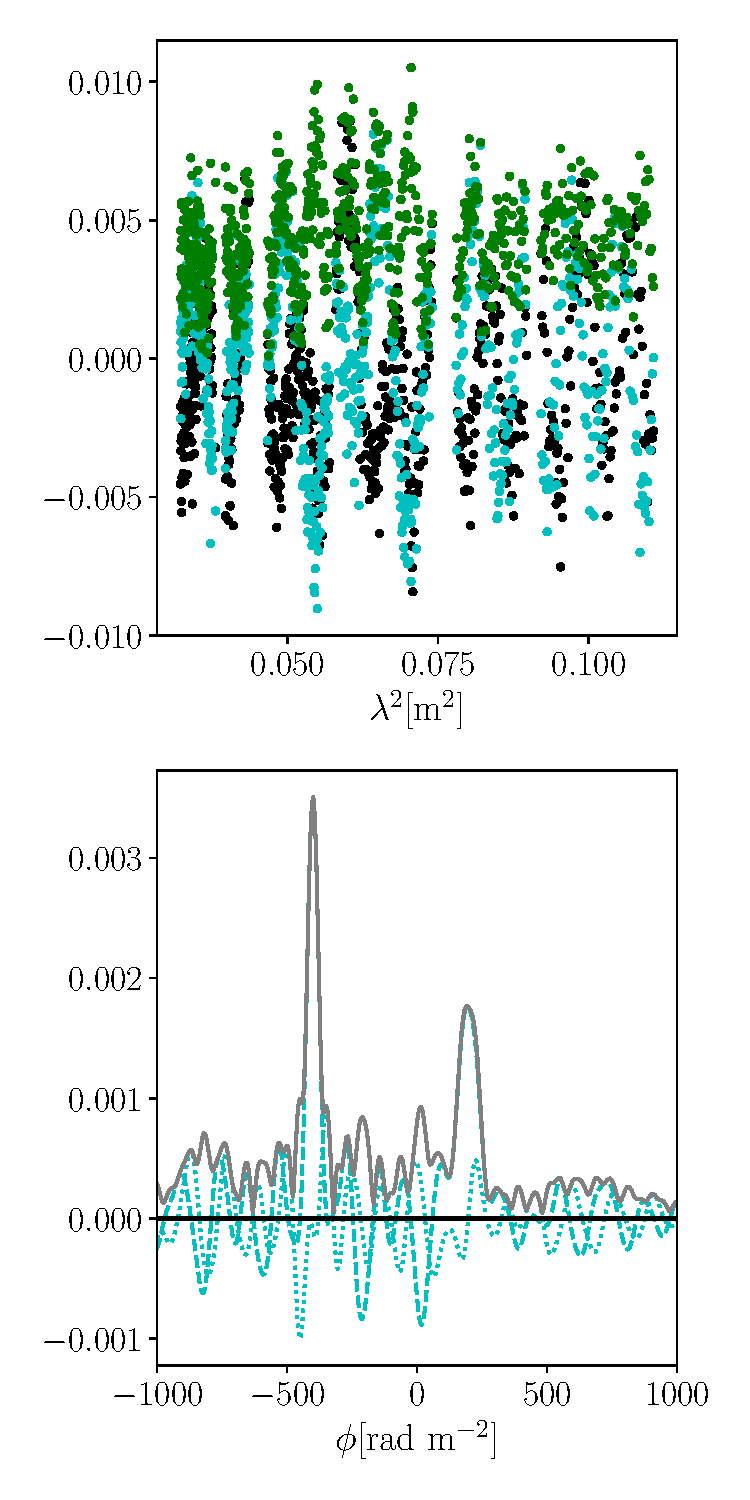
\includegraphics[width=\textwidth]{figures/dataset_features/data_noisy.pdf}
			\caption{1.4~mJy/beam noise}
		\end{subfigure}
	\end{figure}

\end{frame}

\begin{frame}{Galactic RM derotation}
	\begin{columns}[onlytextwidth,t]
		\begin{column}{.5\textwidth}
			\begin{itemize}
				\item The framework applies the derotation directly in $\lambda^2$-space as a phase shift.
			\end{itemize}
			\vspace{1cm}
			\begin{equation*}
				\hat{P}(\lambda^2) = P(\lambda^2)e^{-2i\phi_{\text{GAL}}\lambda^2}
			\end{equation*}
		\end{column}

		\begin{column}{.5\textwidth}
			\begin{figure}
				\centering
				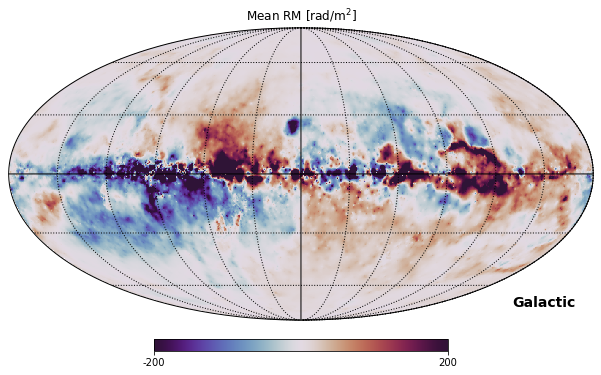
\includegraphics[width=\textwidth]{figures/galactic_derotation/image (2).png}
				\caption*{Mean Galactic RM ~\parencite{faradaysky2020}}
				%\label{fig:my_label}
			\end{figure}
		\end{column}
	\end{columns}
\end{frame}

\begin{frame}{Spectral index correction}
	\begin{columns}[onlytextwidth,t]
		\begin{column}{.5\textwidth}
			\begin{equation*}
				F(\phi) = \frac{1}{K}\int_{-\infty}^{\infty}{W(\lambda^2)\frac{P(\lambda^2)}{s(\lambda^2)} {\rm e}^{-2i\phi \lambda^2}~{\rm d}\lambda^2 }
			\end{equation*}

			\begin{equation*}
				s(\lambda^2) = \frac{I(\lambda^2)}{I(\lambda^2_0)} = \biggl(\frac{\lambda^2}{\lambda^2_0}\biggr)^{-\alpha/2}
			\end{equation*}
			\vspace{1cm}
			\begin{itemize}
				\item ~\cite{brentjens}
				\item For real data we can use FITS/CASA spectral index images
			\end{itemize}
		\end{column}

		\begin{column}{.5\textwidth}
			% Add lambda^2 plots before and after spectral index correction
			\begin{figure}
				\centering
				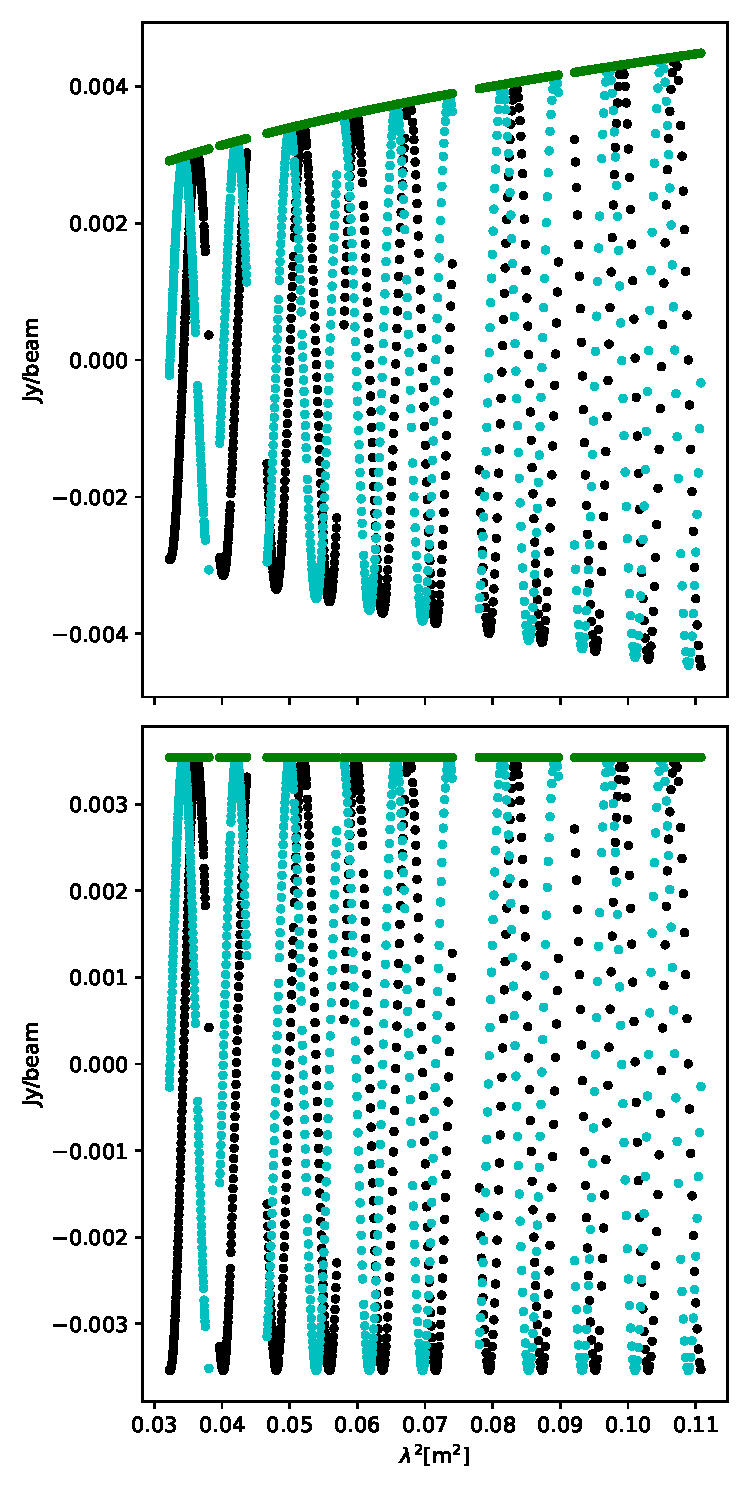
\includegraphics[width=.4\textwidth]{figures/dataset_features/spectral_index_correction.pdf}
				\caption*{$\lambda^2$-space before and after spectral index correction}
				%\label{fig:my_label}
			\end{figure}
		\end{column}

	\end{columns}
\end{frame}

\begin{frame}{Compressed sensing reconstruction}
	\scriptsize
	\begin{columns}[onlytextwidth,t]
		\begin{column}{.5\textwidth}
			\begin{itemize}
				\item Technique that aims to solve inverse problems
				\item Finds the sparsest signal that is consistent with the measurements and to a specific constraint.
			\end{itemize}

			\begin{align*}
				\phi = \argmin_x ||Ax-b||_2^2 + \lambda ||x||_1
			\end{align*}

			\begin{itemize}
				\item $A$: Measurement matrix (Fourier transform)
				\item $b$: Observed data
				\item $x$: Signal or a sparse representation of it.
			\end{itemize}

			\begin{align*}
				x=\sum_i^N c_i\phi_i.
			\end{align*}
		\end{column}

		\begin{column}{.5\textwidth}
			\vspace{1.5cm}
			\begin{figure}
				\centering
				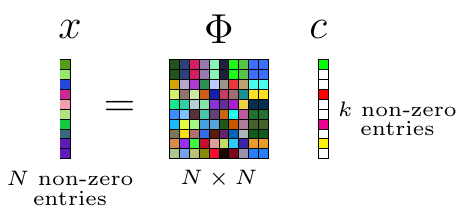
\includegraphics[width=\textwidth]{figures/compressed_sensing.png}
			\end{figure}
		\end{column}

	\end{columns}
\end{frame}

\begin{frame}{Compressed sensing example}
	% Example of compressed sensing for a LOS
	\begin{figure}
		\centering
		\begin{subfigure}{\textwidth}
			\centering
			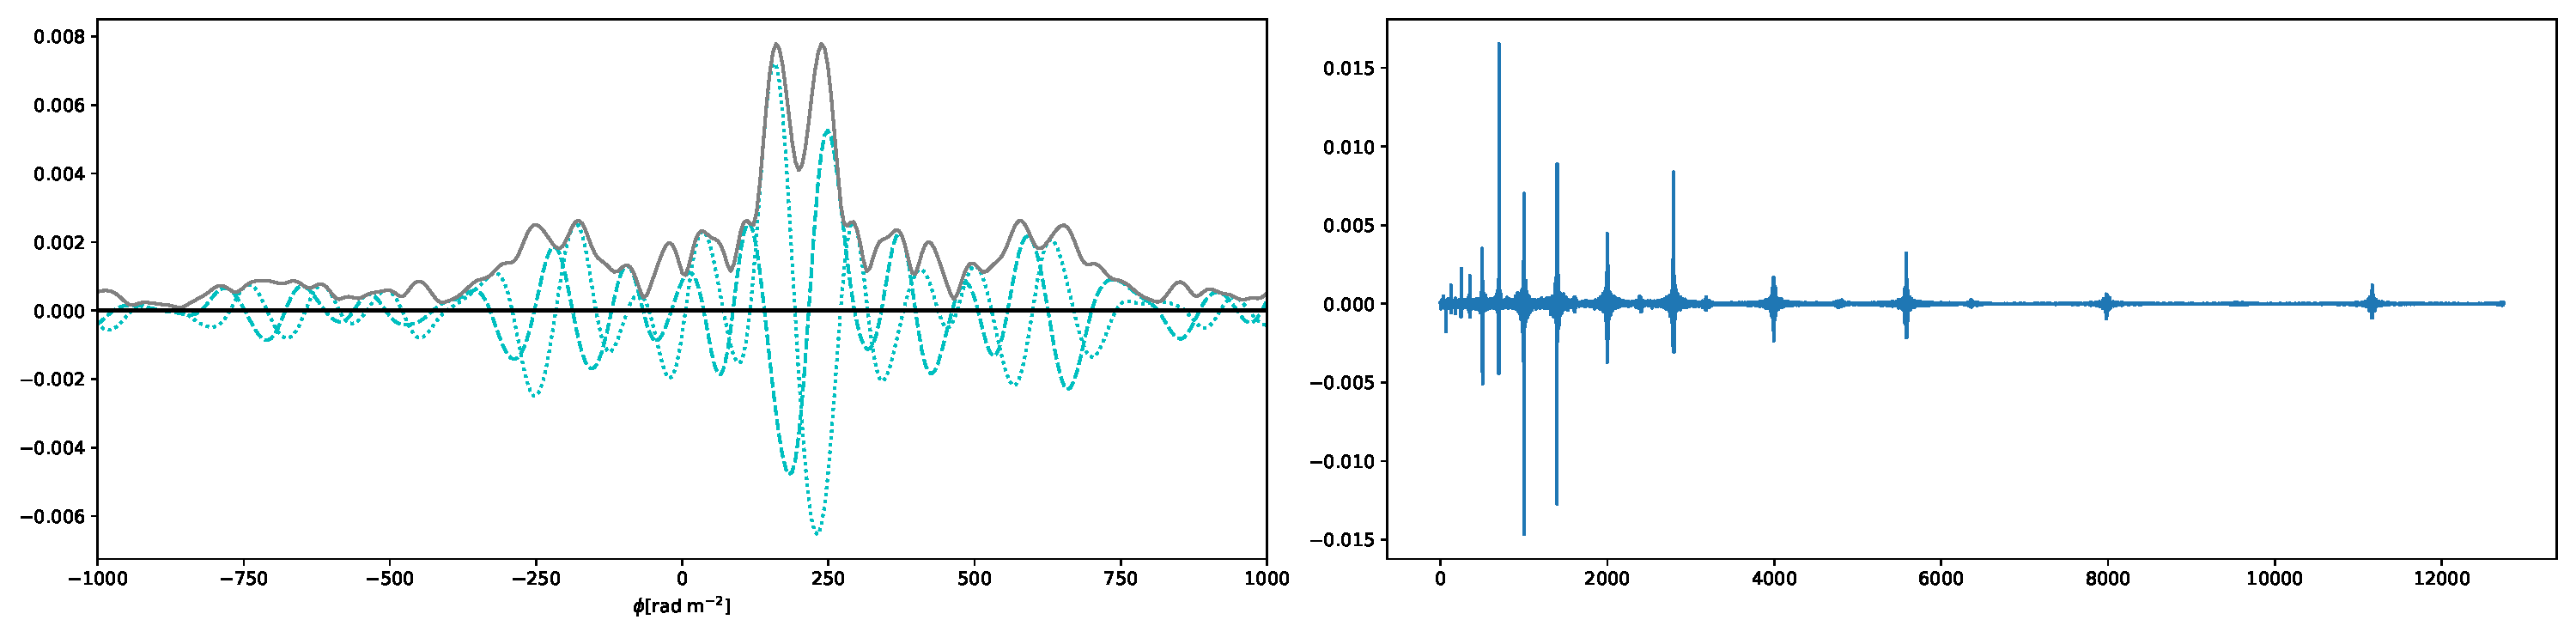
\includegraphics[width=.9\textwidth]{figures/cs/cs_before.pdf}
			\caption{Dirty FD spectrum and coefficient representation}
		\end{subfigure}

		\begin{subfigure}{\textwidth}
			\centering
			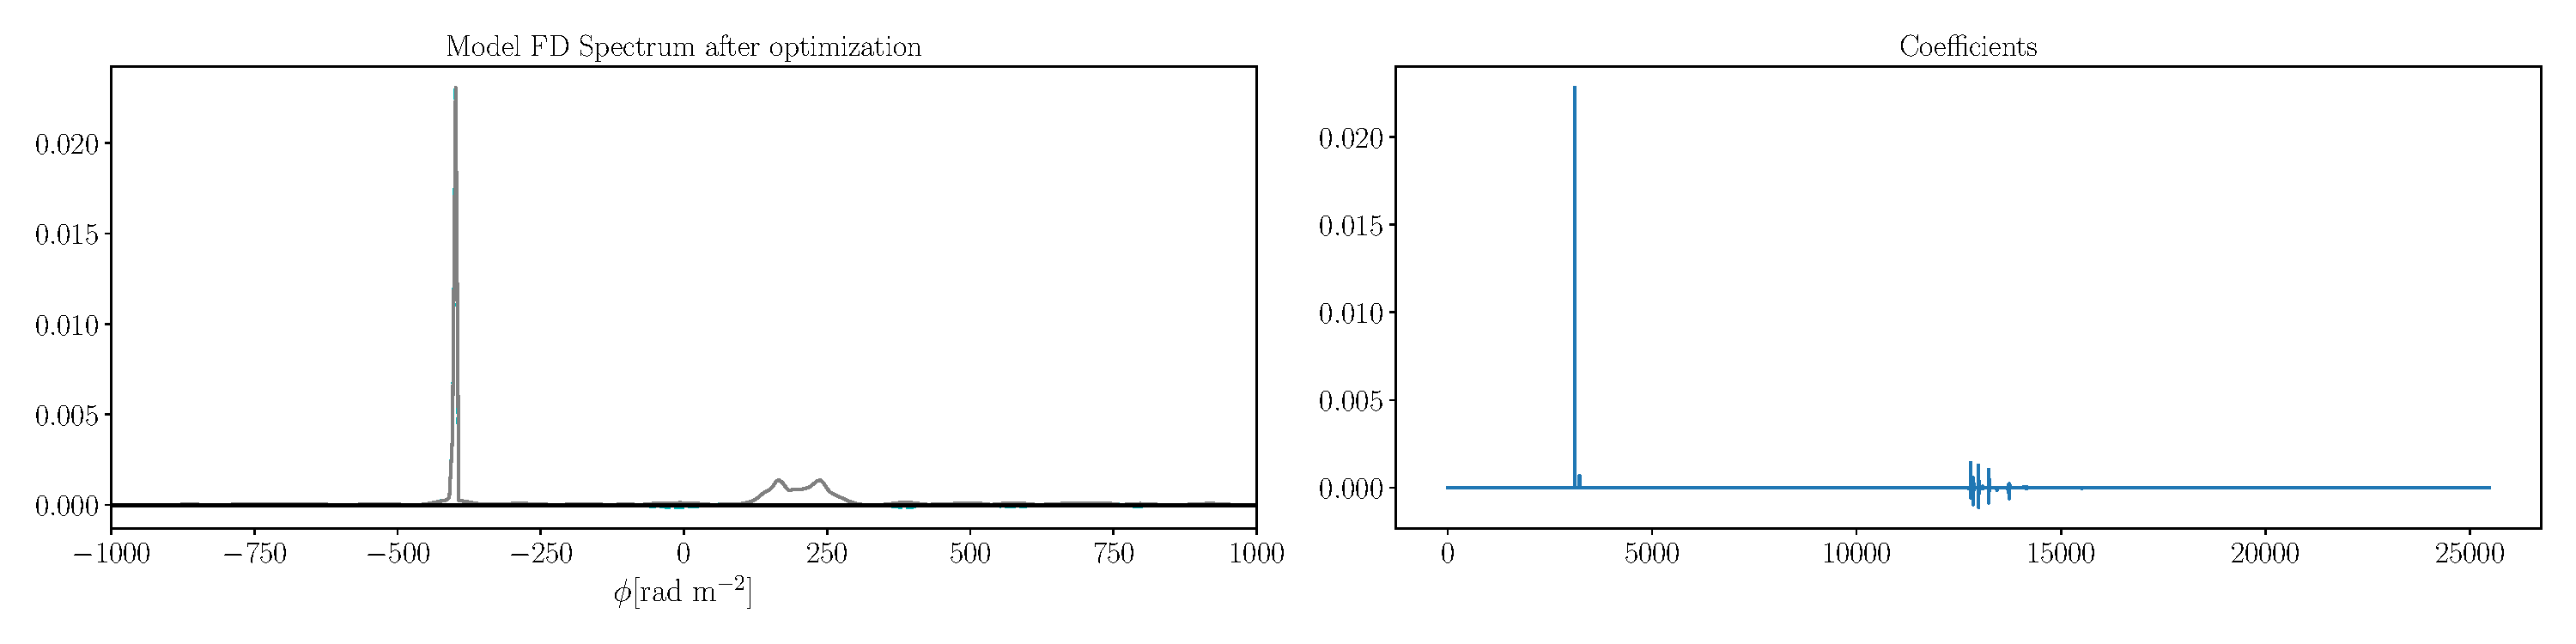
\includegraphics[width=.9\textwidth]{figures/cs/cs_after.pdf}
			\caption{Model FD spectrum and sparse representation (note sparsity of coefficients!)}
		\end{subfigure}
	\end{figure}
\end{frame}

%\begin{frame}{Multiple regularizations}
%    \begin{figure}
%        \centering
%
%        \begin{subfigure}{0.3\textwidth}
%            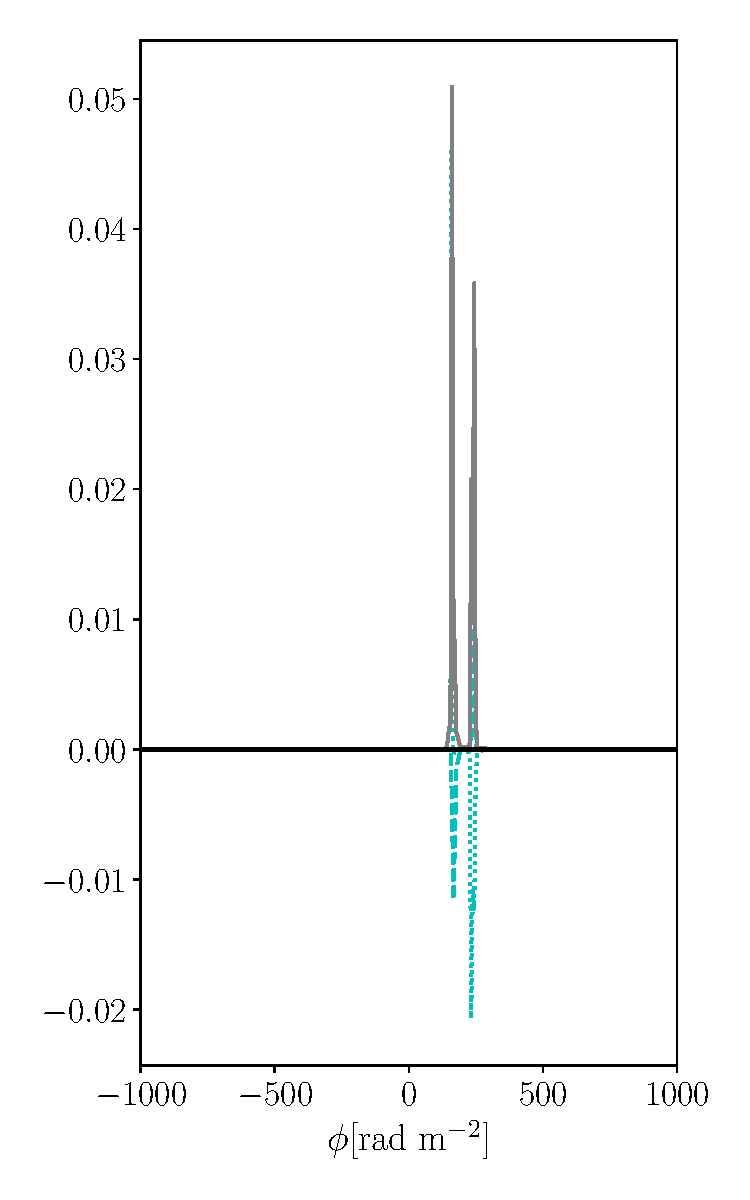
\includegraphics[width=\textwidth]{figures/regularizations/cs_reg_l1.pdf}
%            \caption{L1}
%        \end{subfigure}
%        \begin{subfigure}{0.3\textwidth}
%            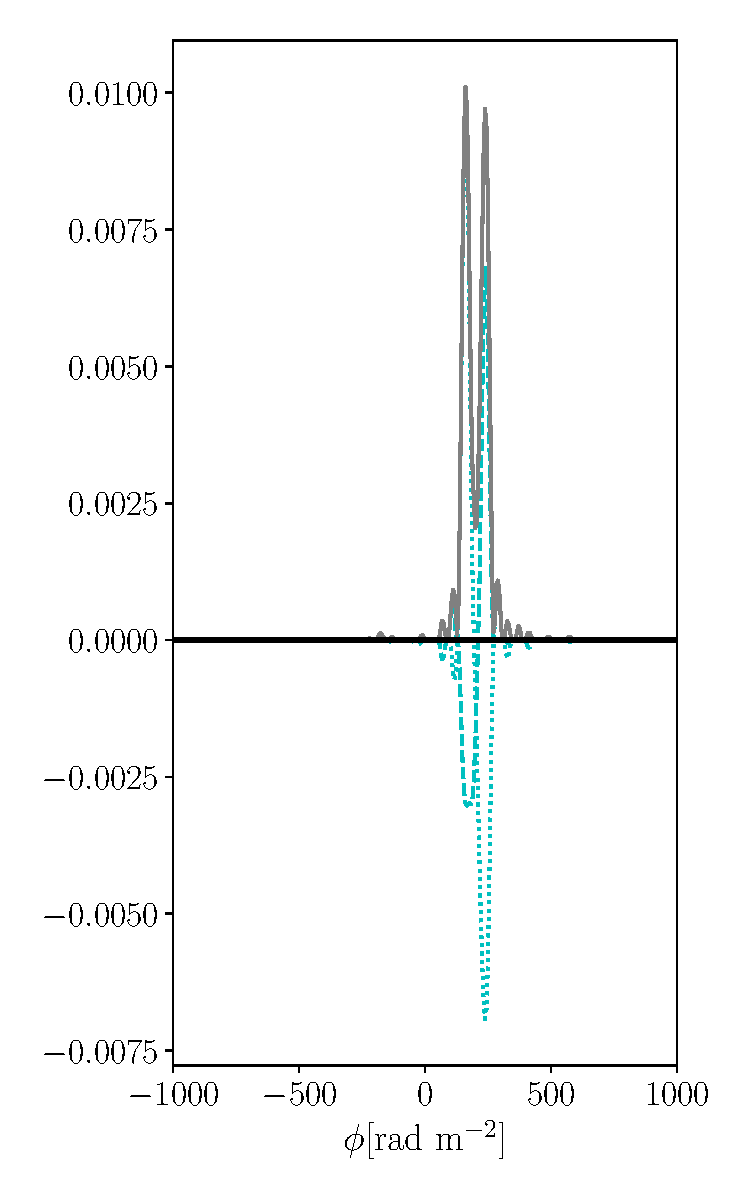
\includegraphics[width=\textwidth]{figures/regularizations/cs_reg_l1tsv.pd%f}
%            \caption{L1+TSV}
%        \end{subfigure}
%        \begin{subfigure}{0.3\textwidth}
%            %\vspace{0.1cm}
%            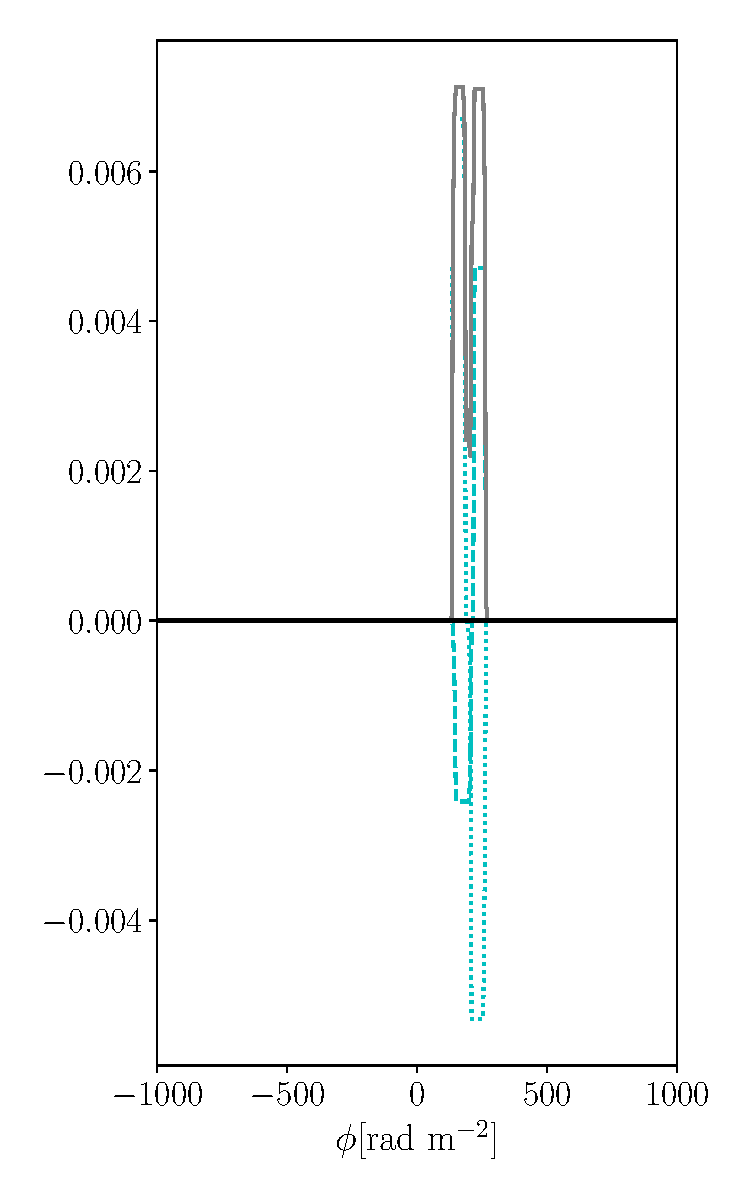
\includegraphics[width=\textwidth]{figures/regularizations/cs_reg_l1tv.pdf}
%            \caption{L1+TV}
%        \end{subfigure}
%    \end{figure}
%\end{frame}

\begin{frame}<0>{Wavelet and performance evaluation}
	\begin{figure}
		\centering
		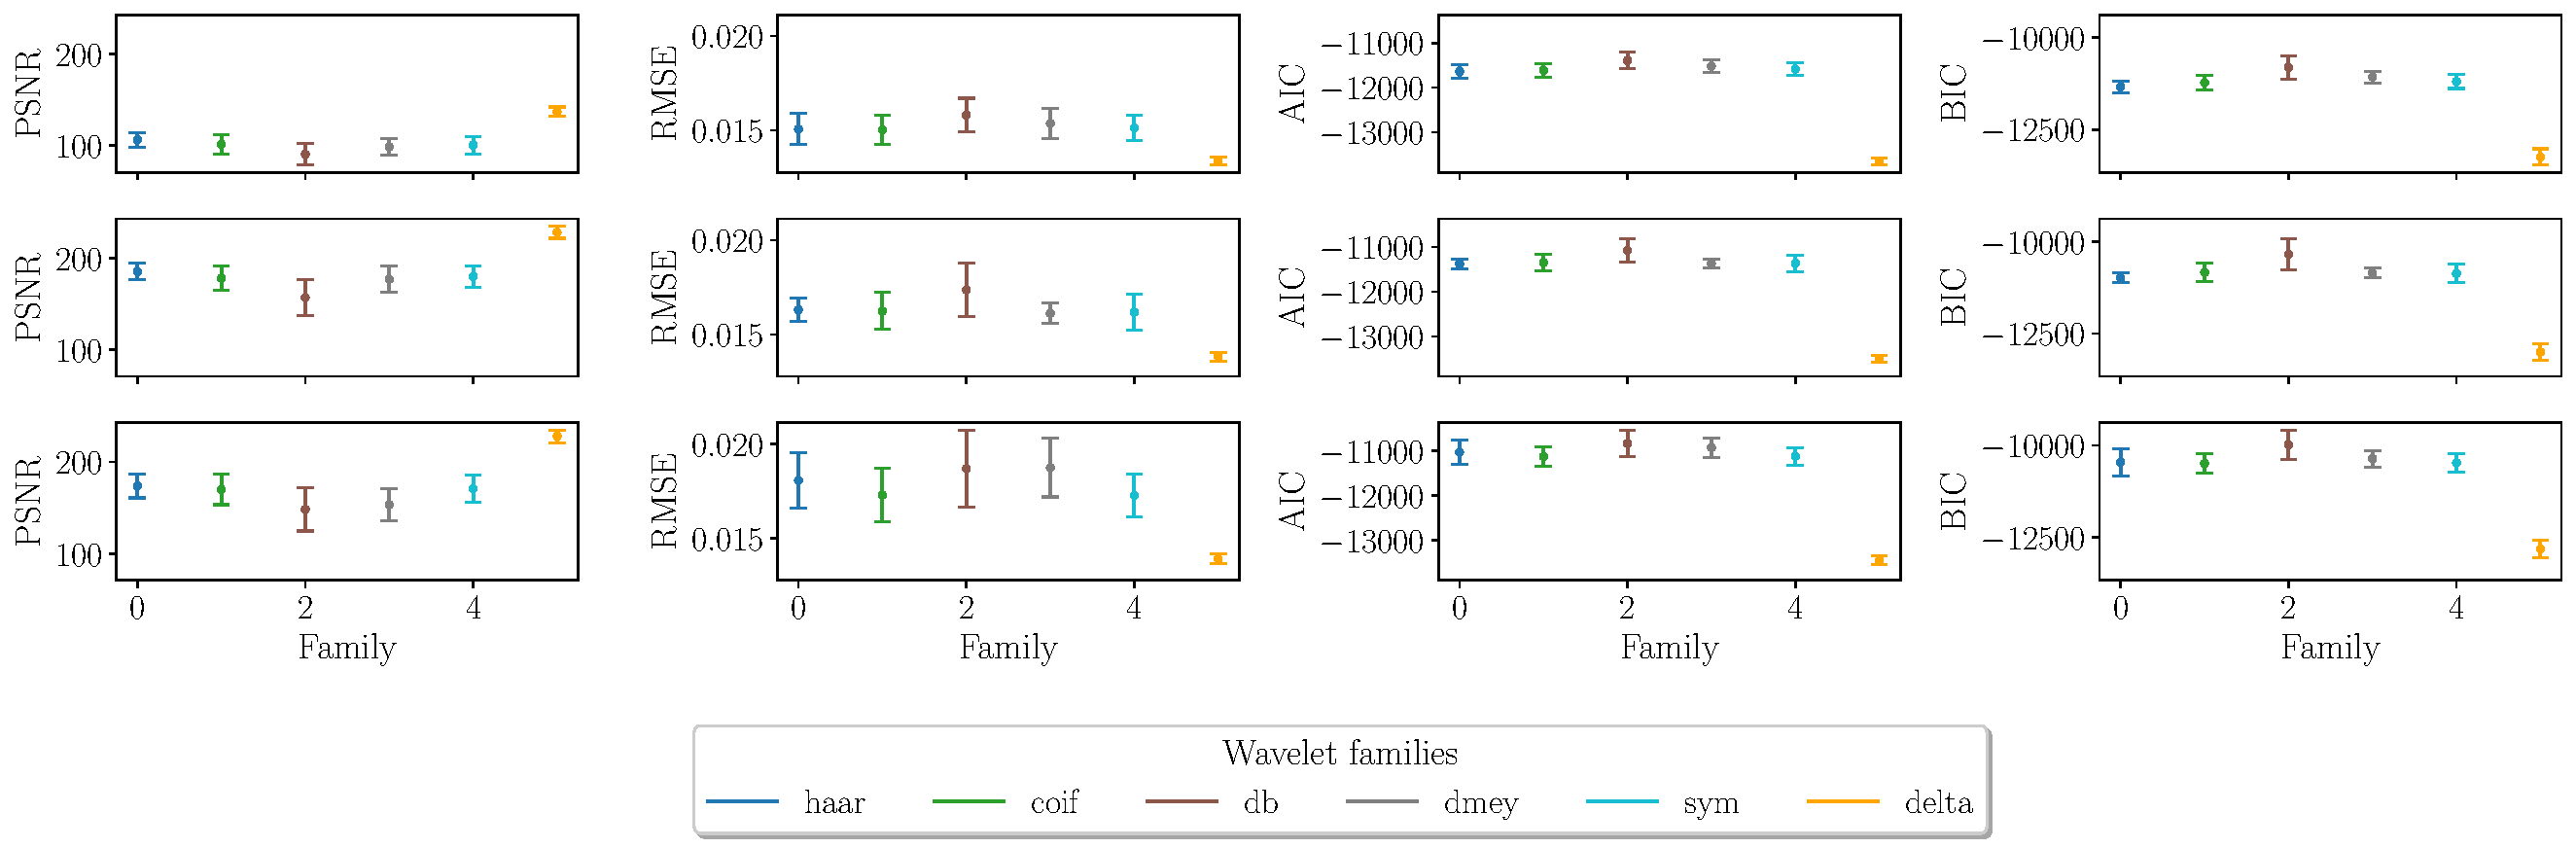
\includegraphics[width=\textwidth]{figures/wavelets/families_wavelets_meerkat.pdf}
		\caption*{Peak signal-to-noise ratio, root mean squared error, Akaike and Bayesian Information criterias for thin, thick and mixed sources.}

		%\begin{subfigure}{\textwidth}
		%    \centering
		%    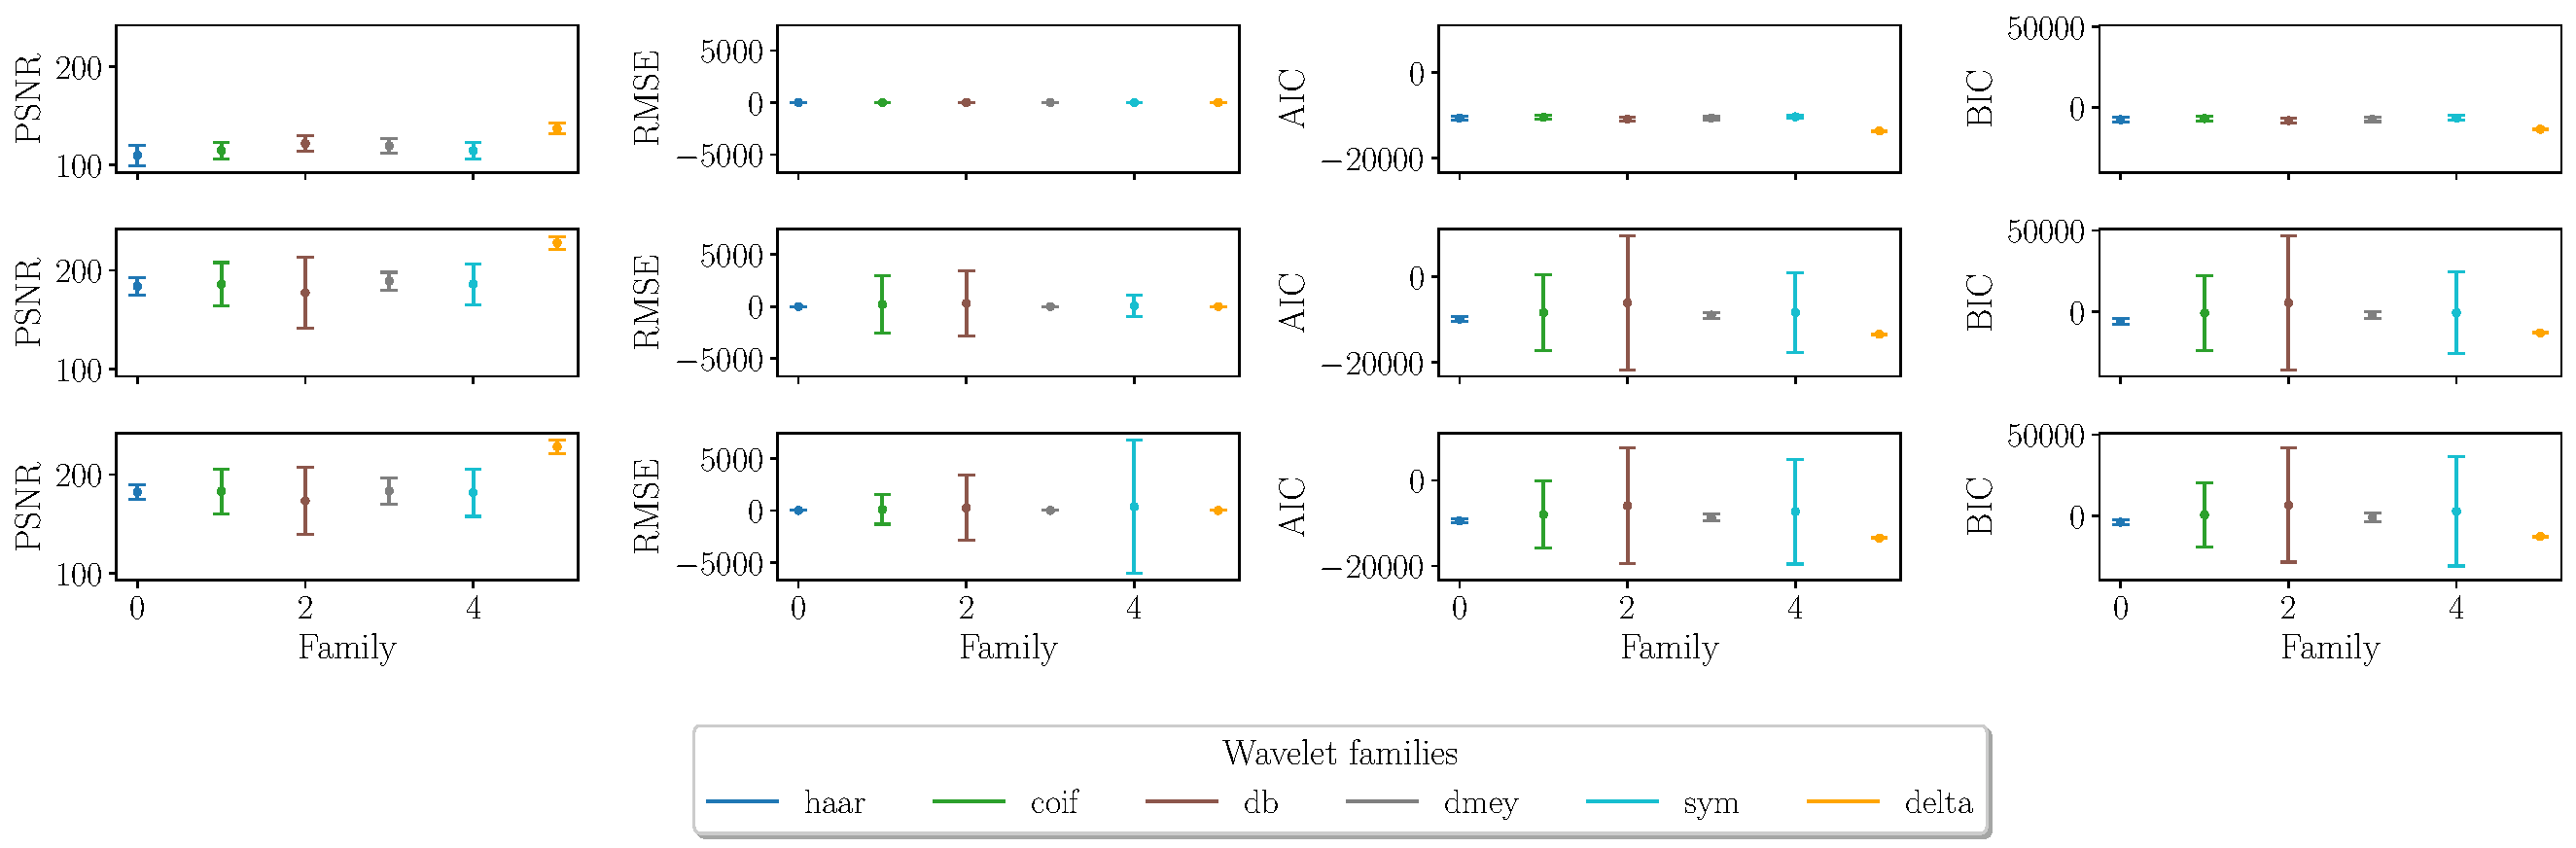
\includegraphics[width=0.8\textwidth]{figures/wavelets/families_undecimatedwavelets_meerkat.pdf}
		%\end{subfigure}
	\end{figure}
\end{frame}


\begin{frame}{Preliminary results in the XMMLSS-12 early science field}

	\begin{figure}
		\centering
		\begin{subfigure}{\textwidth}
			\centering
			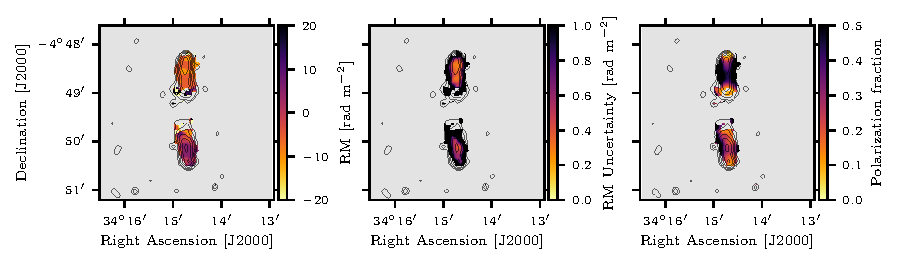
\includegraphics[width=0.85\textwidth]{figures/plot_rm.pdf}
			%\caption{Firts subfigure.}
			%\label{fig:first}
		\end{subfigure}
		\begin{subfigure}{\textwidth}
			\centering
			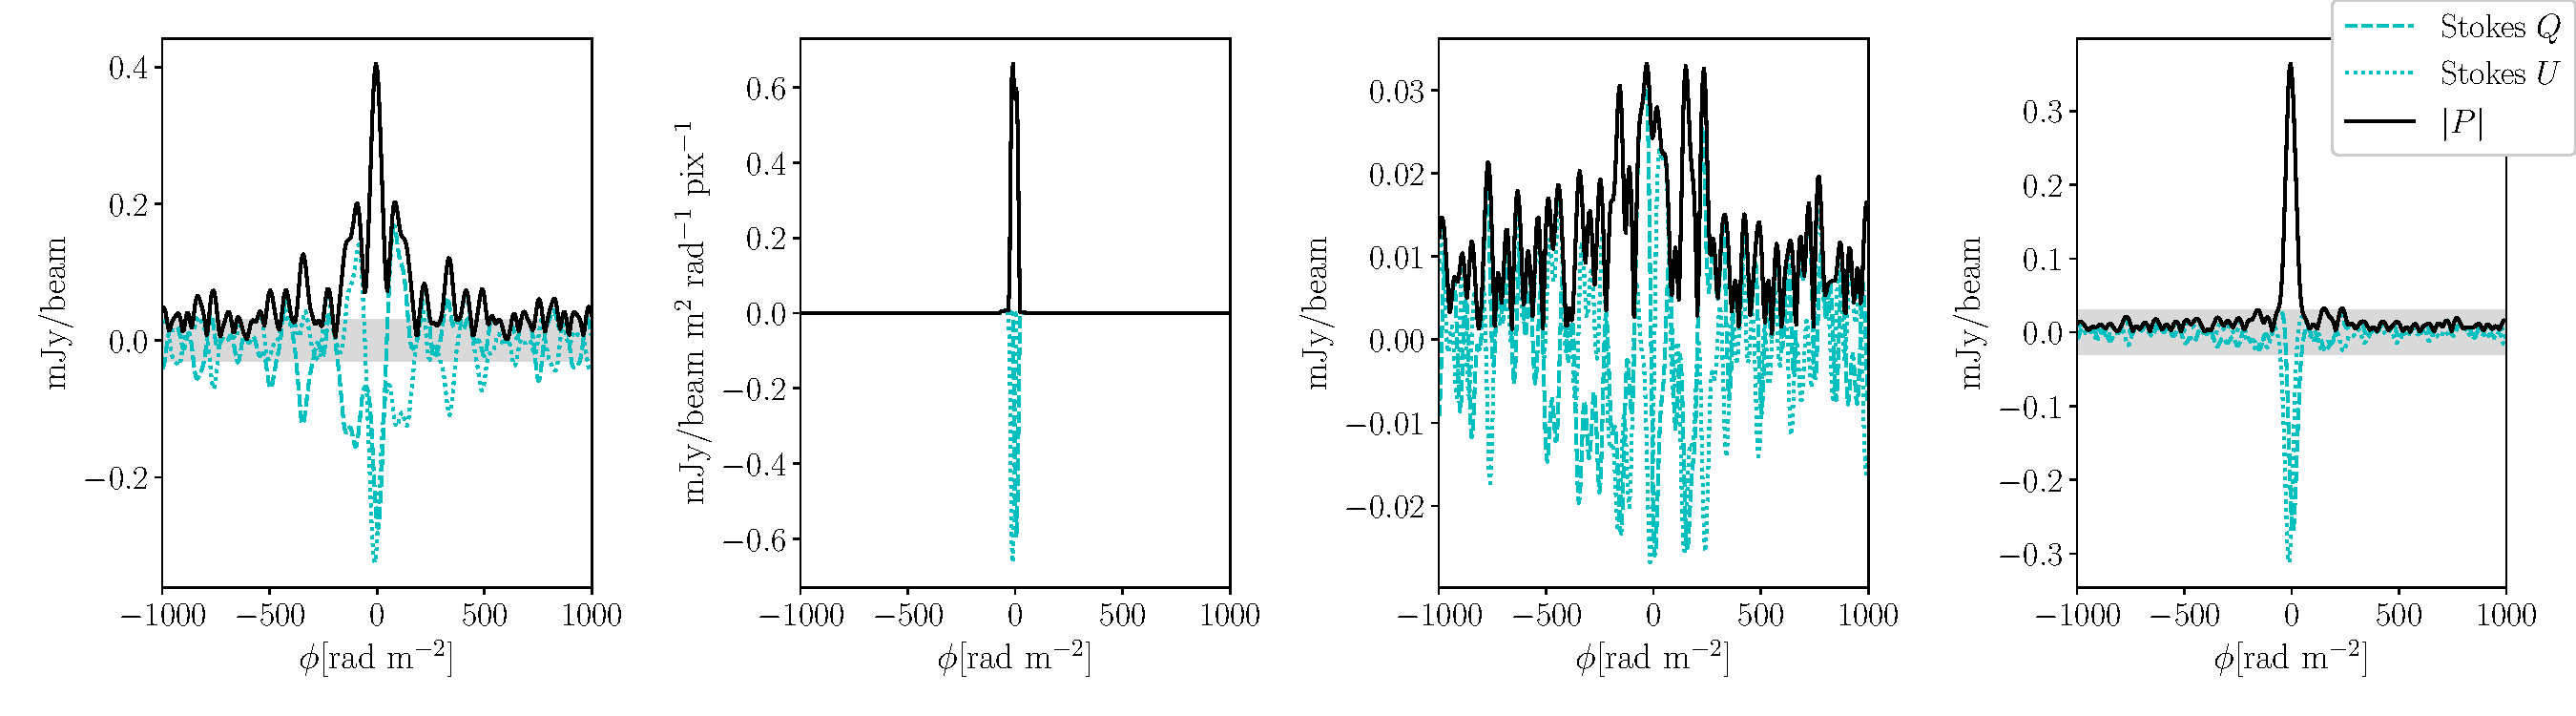
\includegraphics[width=0.85\textwidth]{figures/los.pdf}
			\caption{Dirty, model, residuals and restored Faraday depth spectra.}
			%\label{fig:second}
		\end{subfigure}

	\end{figure}
\end{frame}

\begin{frame}{Conclusions}
	\begin{itemize}
		\item We have already demonstrated this method with real data ~\parencite{a1314-csromer} (\href{https://arxiv.org/abs/2205.01413}{\texttt{arXiv 2205.01413}}).
		\item We need to apply this method to all the MIGHTEE-POL survey maps
		\item Add {\tt cs-romer} RM and RM uncertainties to the MIGHTEE catalog
		\item Compare the RM values with QU-fitting and naive RM-Synthesis
		\item We need to incorporate big data and big computing packages such as {\tt dask} and {\tt cupy} to {\tt cs-romer}
	\end{itemize}
\end{frame}

\end{document}
